
After testing and simulating the system design in the simulation software, construction and installation of individual systems begin.
This section explains the installation and configuration of each system with their individual components, while also explaining their functionality.

\subsection{Detection marker}
\label{subsec:marker}
Detection marker is a $15\times13$ 200 mm pattern that is used to determine the pose of a system placed in the workcell using the \hyperref[acro:VISOR]{VISOR}\textsuperscript{\textregistered} vision sensor
mounted on the \hyperref[acro:KR]{KR}. The pose represents the position and orientation in \hyperref[acro:3D]{3D} space. In total, there are ten markers in the robotic workcell.
One each for bending machine unit and unloading station; and ten markers for the storage station.

\begin{figure}[h]
    \centering
    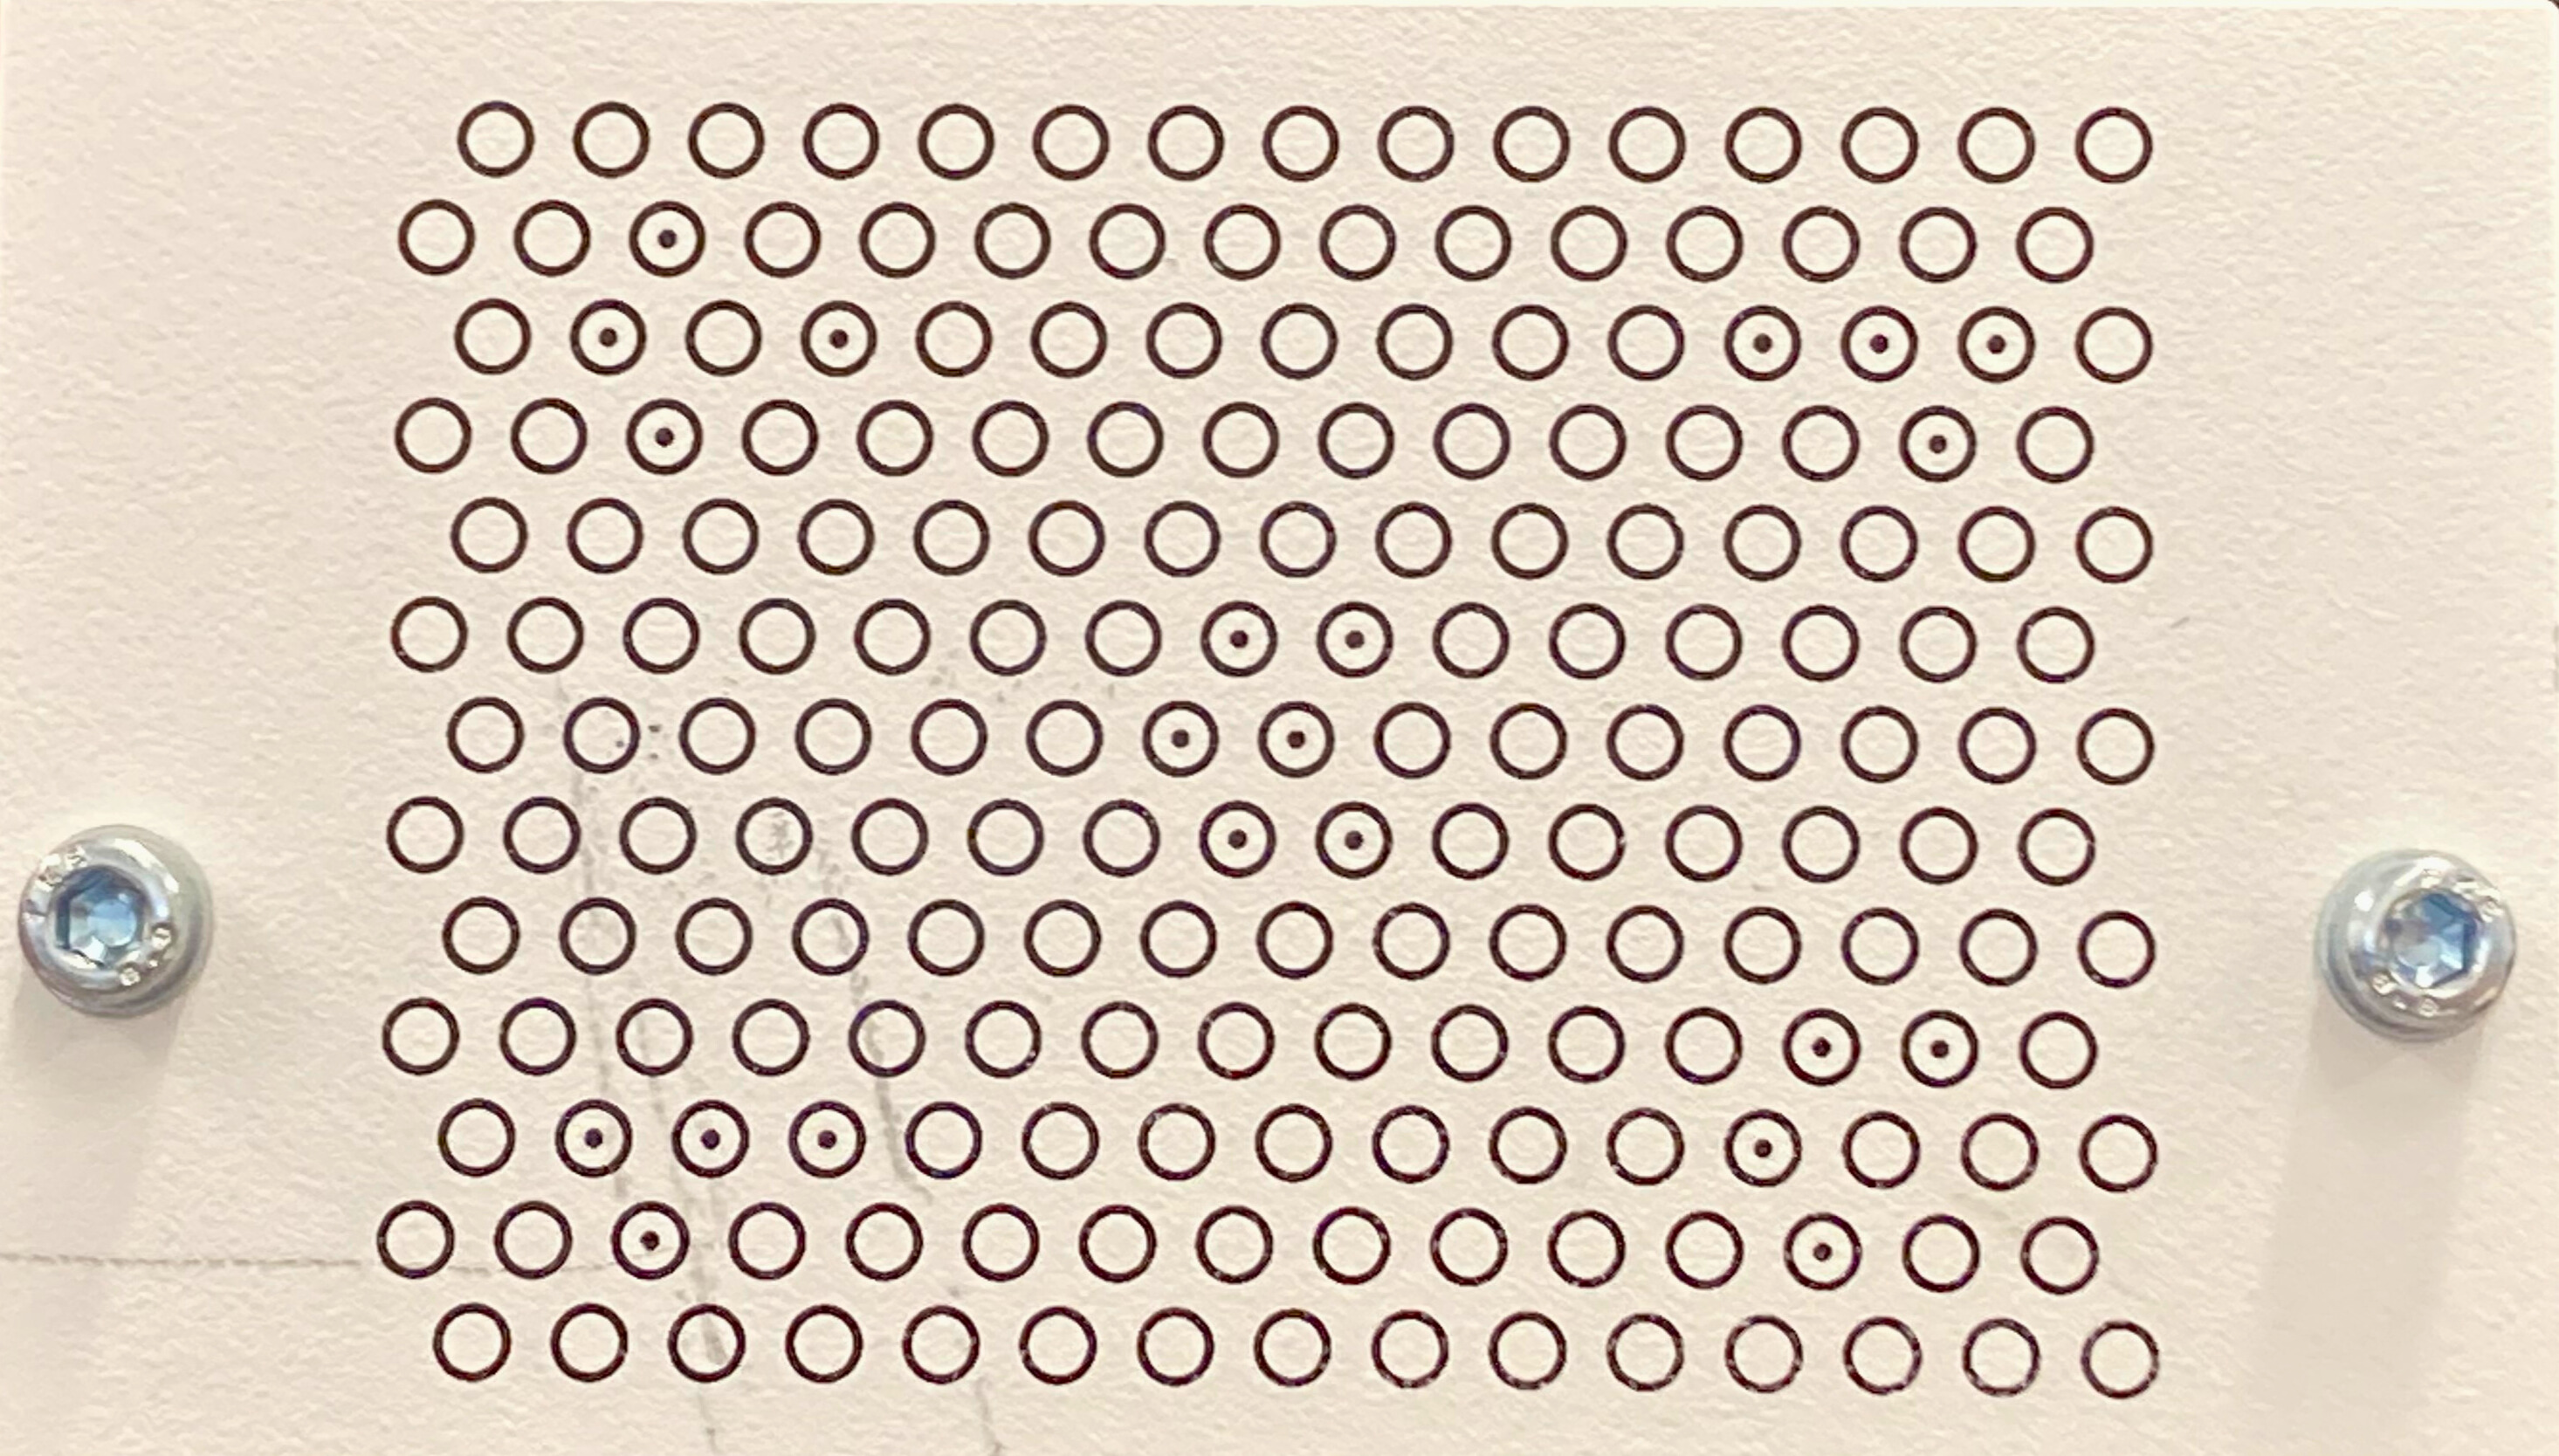
\includegraphics[width=0.5\textwidth]{figures/detection-marker.png}
    \caption{Detection marker}
    \label{fig:marker}
\end{figure}

In addition to get the pose, detection marker is used as calibration plate for auto calibration of camera \textit{w.r.t.} \hyperref[acro:TCP]{TCP}.


\subsection{Bending machine unit}
\label{subsec:bending-machine}
Bending machine is set to operate automatically by controlling the foot pedal with \hyperref[acro:PLC]{PLC}.
To automate the bending process, several devices and components are installed on the bending machine.
Bending machine is operated freely up to a certain point \textit{i.e.} without any pressure and only starts
applying pressure when it is in contact with the sheet metal part.
Figure \ref{fig:bending_machine} shows these components.


\subsubsection{Marker}
\label{subsubsec:marker}
Detection marker mounted on the bending machine. This pose is used as reference frame for all three bending stations.
Since the bending machine is fixed, this marker is also used for auto calibration of the robotic camera.


\begin{figure}[h]
    \centering
    \includegraphics[width=1\textwidth]{figures/bending-machine.png}
    \caption{\hyperref[acro:AMADA]{AMADA} Bending Machine. 1) Marker  2) Bending machine open height measurement sensor 3) Bending station 4) Terminal fixture 5) Laser monitoring}
    \label{fig:bending_machine}
\end{figure}

\subsubsection{Bending machine open height measurement sensor}
\label{subsubsec:laser-sensor}

It is important to know exactly the current open height of the bending machine.
This value tells the \hyperref[acro:KR]{KR} to open the pneumatic parallel gripper as sheet starts bending at a bending station to avoid any deformation in the sheet.
Once the bending is complete, the \hyperref[acro:KR]{KR} can move out safely without any collision if a set-point on the open height is reached.

For this, a laser sensor is mounted on the bending machine which measures the open height of the bending machine.
The sensor values are sent to the \hyperref[acro:PLC]{PLC}. \hyperref[acro:KR]{KR} makes decision to do bending operation based on this laser sensor value.


\subsubsection{Bending station}
\label{subsubsec:bending-station}
There are three bending stations in the bending machine. Each bending station has a different set of punch and die.
Bending station 1 is used to achieve a bending of 90\textdegree. Bending station 2 bends the sheet metal part at an angle of 135\textdegree.
And finally, bending station is used to press down the sheet and make it flat.

\begin{figure}[h]
    \centering
    \includegraphics[width=0.7\textwidth]{figures/bending-station.png}
    \caption{Three bending stations for the bending operation}
    \label{fig:bending-station}
\end{figure}

These three stations are enough for the sheet bending operation. \hyperref[acro:KR]{KR1410} will take the sheet metal part to one of these bending station
to perform a bending of a particular angle. A sheet metal part could require the use of one or more of these bending stations.

\subsubsection{Terminal Fixture}
The bending machine comes with a terminal which is used to operate the bending machine. However, this terminal is free to rotate and move.
It is required to fix the movement of terminal, so that terminal operating robot could operate reliably. The fixtures made from aluminum profiles fixes the bending machine
terminal.


\subsection{Robot unit}
\label{subsec:robot-unit}
The robot unit consists of three assemblies: a base, a robot and an end-effector. (Figure \ref{fig:robot-installation}).
The robot is a manipulator from kassow robots with pneumatic parallel grippers as the end-effector.
Pneumatic gripper is controlled by PLC. \hyperref[acro:VISOR]{VISOR\textsuperscript{\textregistered}} camera is also mounted on the tool-IO which is used for robotic perception.


\begin{figure}[h]
    \centering
    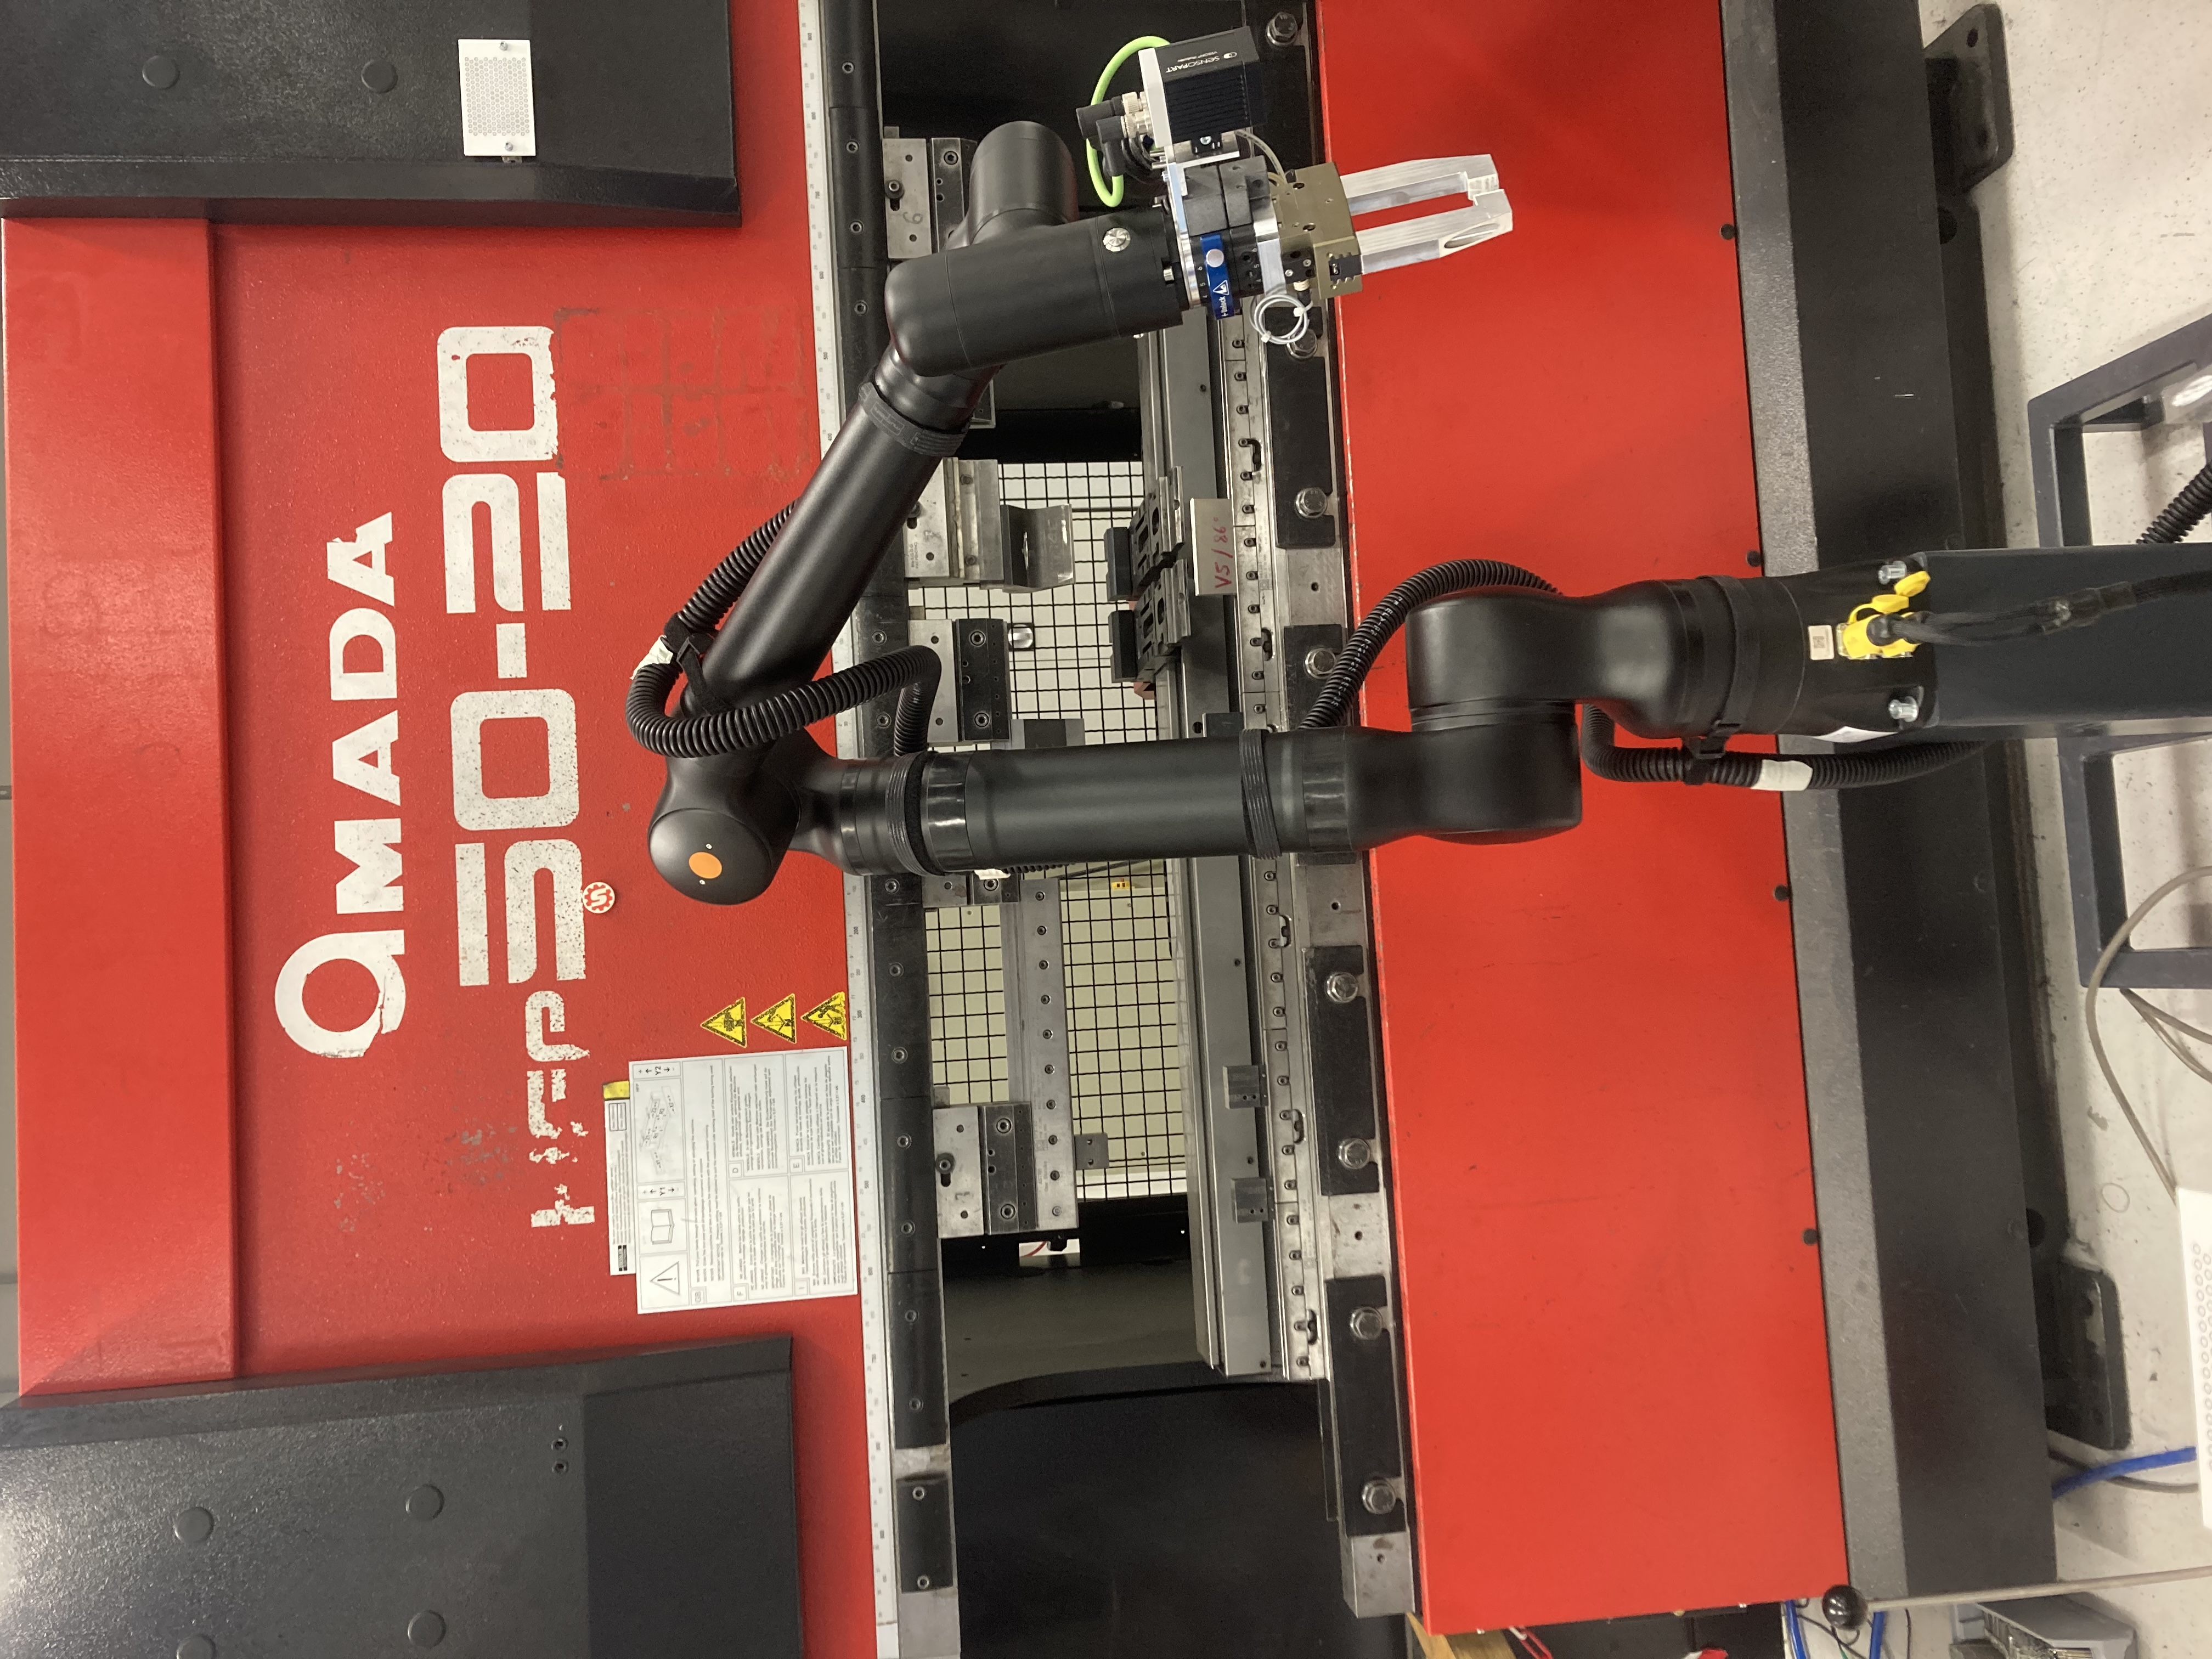
\includegraphics[width=1\textwidth]{figures/handling-robot.png}
    \caption{Three bending stations for the bending operation}
    \caption{Components of the robot unit: 1) robot base 2) KR1410 manipulator 3) manual quick-change system 4) robotic gripper 5) robotic camera}
    \label{fig:robot-installation}
\end{figure}



\subsubsection{Robot base}
The base is a simple welded construction made of steel. The choice of steel material ensures that the base has
sufficient dead weight so that it can be transported together with the robot and gripper using a pallet
truck without the risk of tipping over. During operation, the robot unit is fixed to the floor with four M12
screws. 

\subsubsection{KR1410 manipulator}
The robot used is a 7-axis robot from \textbf{Kassow Robots} with model KR1410. This robot model fulfills the requirements defined in 
the section \ref{sec:requirements}. Simulations have shown that this robot is above to reach even the lowest drawers of the shelf of the
storage station. Two full rotations (720\textdegree) of five out of seven joints allows complex motions in limited space.
A flexible conduit containing pneumatic hose for the pneumatic parallel gripper and communication cabel for the camera goes around the manipulator to reach the end-effector.



\subsubsection{Manual quick-change system}
The gripper is attached to a manual quick-change
system. The manual quick-change system makes it possible to exchange different gripper
designs in a short time and without increased effort if required for a sheet metal part type. Sheet metal
part is folded into something like a box. The quick-change system also has an electric and pneumatic power feed-through, which ensures simple,
user-friendly changeover.

\subsubsection{Robotic Gripper}
The gripper is a Schunk pneumatic parallel gripper. It is powered and controlled by the Tool-IO board on the KR1410.
The robotic gripper grips an object with an applied pressure of five bar. This is enough to hold the sheet metal part
in place during motion of the arm. 
The fingers are made from aluminium material and finger tips are 3D printed using a \hyperref[acro:FDM]{FDM} printer. The tips are worn out
after some period of time, but are easily replacable by 3D printing.
In the program tree, TCP is set at the center of the finger tips of the robotic gripper.


\subsubsection{Robotic Camera}
A camera system is installed on the robot itself. This is used to determine the relative
position between the robot unit and the unloading station, bending machine and storage station using the markers
and between the robot unit and the sheet metal part (when it is first made available at the
unloading station or is gripped) using features on the sheet metal part.
As the working distance of this camera is large, using external light source is required to protect against ambient light. 
This is because light reflections or changing extraneous light can distort evaluation results.


\subsection{Storage station}
\label{subsec:storage-station}
The storage station is a shelf of 10 drawers and is constructed entirely from aluminum profiles.
At the heart of the storage box are the modular drawers, which consist of a universal basic
construction and individual sheet metal part support plates. The basic construction consists
of an aluminum profile frame, two telescopic rails and a locking mechanism, which prevents the
drawer from moving unintentionally when pulled out or pushed in. Due to the greater need for profiles and
connection technology, the costs for this construction method are somewhat higher, but the storage
box can be manufactured precisely as a result, which will have a positive effect on process reliability
later when the sheet metal parts are stored.

\begin{figure}[h]
    \centering
    \begin{subfigure}{0.35\textwidth}
        \centering
        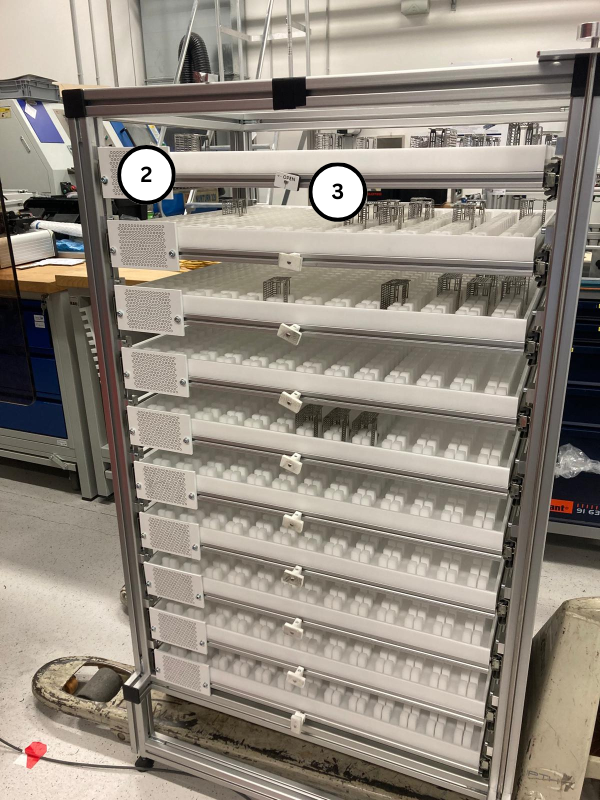
\includegraphics[width=\textwidth]{figures/storage-station-front.png} % Replace with your image file
        \subcaption{front-view}
        \label{fig:storage-station-front}
    \end{subfigure}\hspace{1cm}
    \begin{subfigure}{0.36\textwidth}
        \centering
        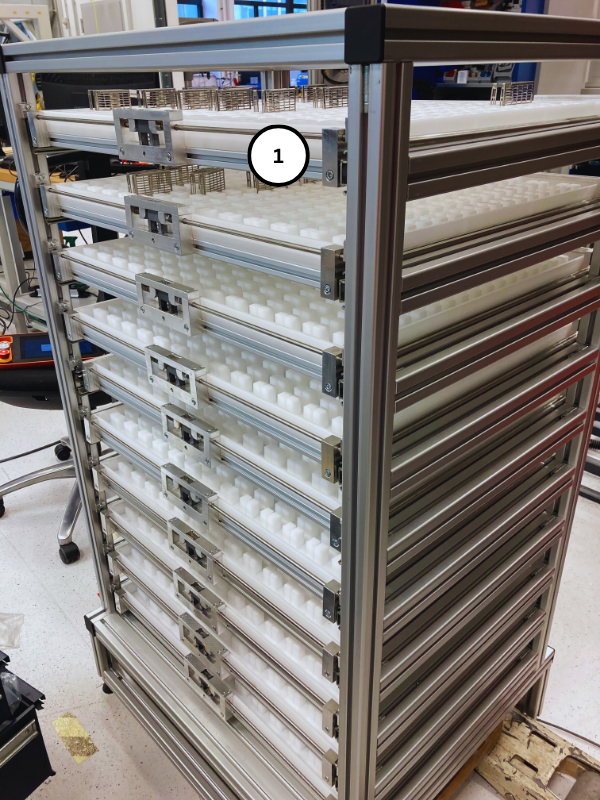
\includegraphics[width=\textwidth]{figures/storage-station-back.png} % Replace with your image file
        \caption{back-view}
        \label{fig:storage-station-back}
    \end{subfigure}
    \caption{Storage station of 10 drawers 1) drawer 2) marker 3) shelf handle}
    \label{fig:storage-station-main}
\end{figure}

The individual drawers could be pulled out using
telescopic rails automatically by the robot. 
The individual drawer is a 30 mm thick plate with regularly arranged recesses,
which enables the finished sheet metal parts to be placed in a defined position for the robot unit. For
weight reasons, plastic was the only material considered and the drawers are printed using \hyperref[acro:AM]{AM}.
Due to the possibility of customizing the sheet metal part carrier plate, the
focus of the design implementation was on designing a carrier plate that can be used for several sheet
metal part variants at the same time. On the one hand, this saves material resources, and on the other
hand, different sheet metal part carrier plates do not have to be kept in stock or the storage boxes do
not always have to be converted when changing products.


Each drawer has its own locking mechanism. This is operated with a handle on the front by turning it
clockwise or anticlockwise. The handle also serves as a gripping object for the robot
unit, by means of which the drawer can be pulled out or pushed in. In addition to this locking mechanism,
each storage box has a locking bar across all drawers. This is intended to serve as an additional
safeguard when the boxes are moved between different factory halls and/or over longer distances
using a forklift truck. In addition, each individual drawer is equipped with a detection marker pattern that is
used to determine the spatial position using the camera on the robot unit. This is required
for the reliable depositing of the sheet metal parts.

\subsection{Unloading station}
\label{subsec:unloading-station}
Figure \ref{fig:unloading-station-main} shows the elementary components of this station.



\begin{enumerate}
    \item A marker is attached to the unloading station through which robot get the exact position of the unloading station.
    
    \begin{figure}[h]
        \centering
        \includegraphics[width=0.9\textwidth]{figures/unloading-station.png}
        \caption{\parbox[t]{12cm}{Unloading station configuration. 1) Marker 2) Gantry 3) Magnetic gripper 4) Gripper 5) Inspection Camera 6) Control cabinets 7) KR1410 Teach pendant holder
        8) SIMATIC HMI}}
        \label{fig:unloading-station-main}
    \end{figure}

    \item Similar to the storage station, the raw sheets are stored on a pull-out drawer. This also consists
    of a universal basic construction and an individual perforated grid plate. Depending on the type of
    sheet metal part, the blanks can be stacked on this perforated grid plate. The sheet metal parts can be
    held in place by means of sheet metal brackets that are screwed to the plate. Telescopic rails are also
    used here. Because the drawer does not have to be opened by a robot, but only by a person, rails with
    integrated locking mechanisms are used. Pulling out the drawer ensures ergonomically simple
    filling. The drawer position is monitored using a position switch. A gantry robot with a working area of $400 \times 1000 \times 250 mm$ is to be used for destacking.
    
    \begin{figure}[h]
        \centering
        \begin{subfigure}{0.5\textwidth}
            \centering
            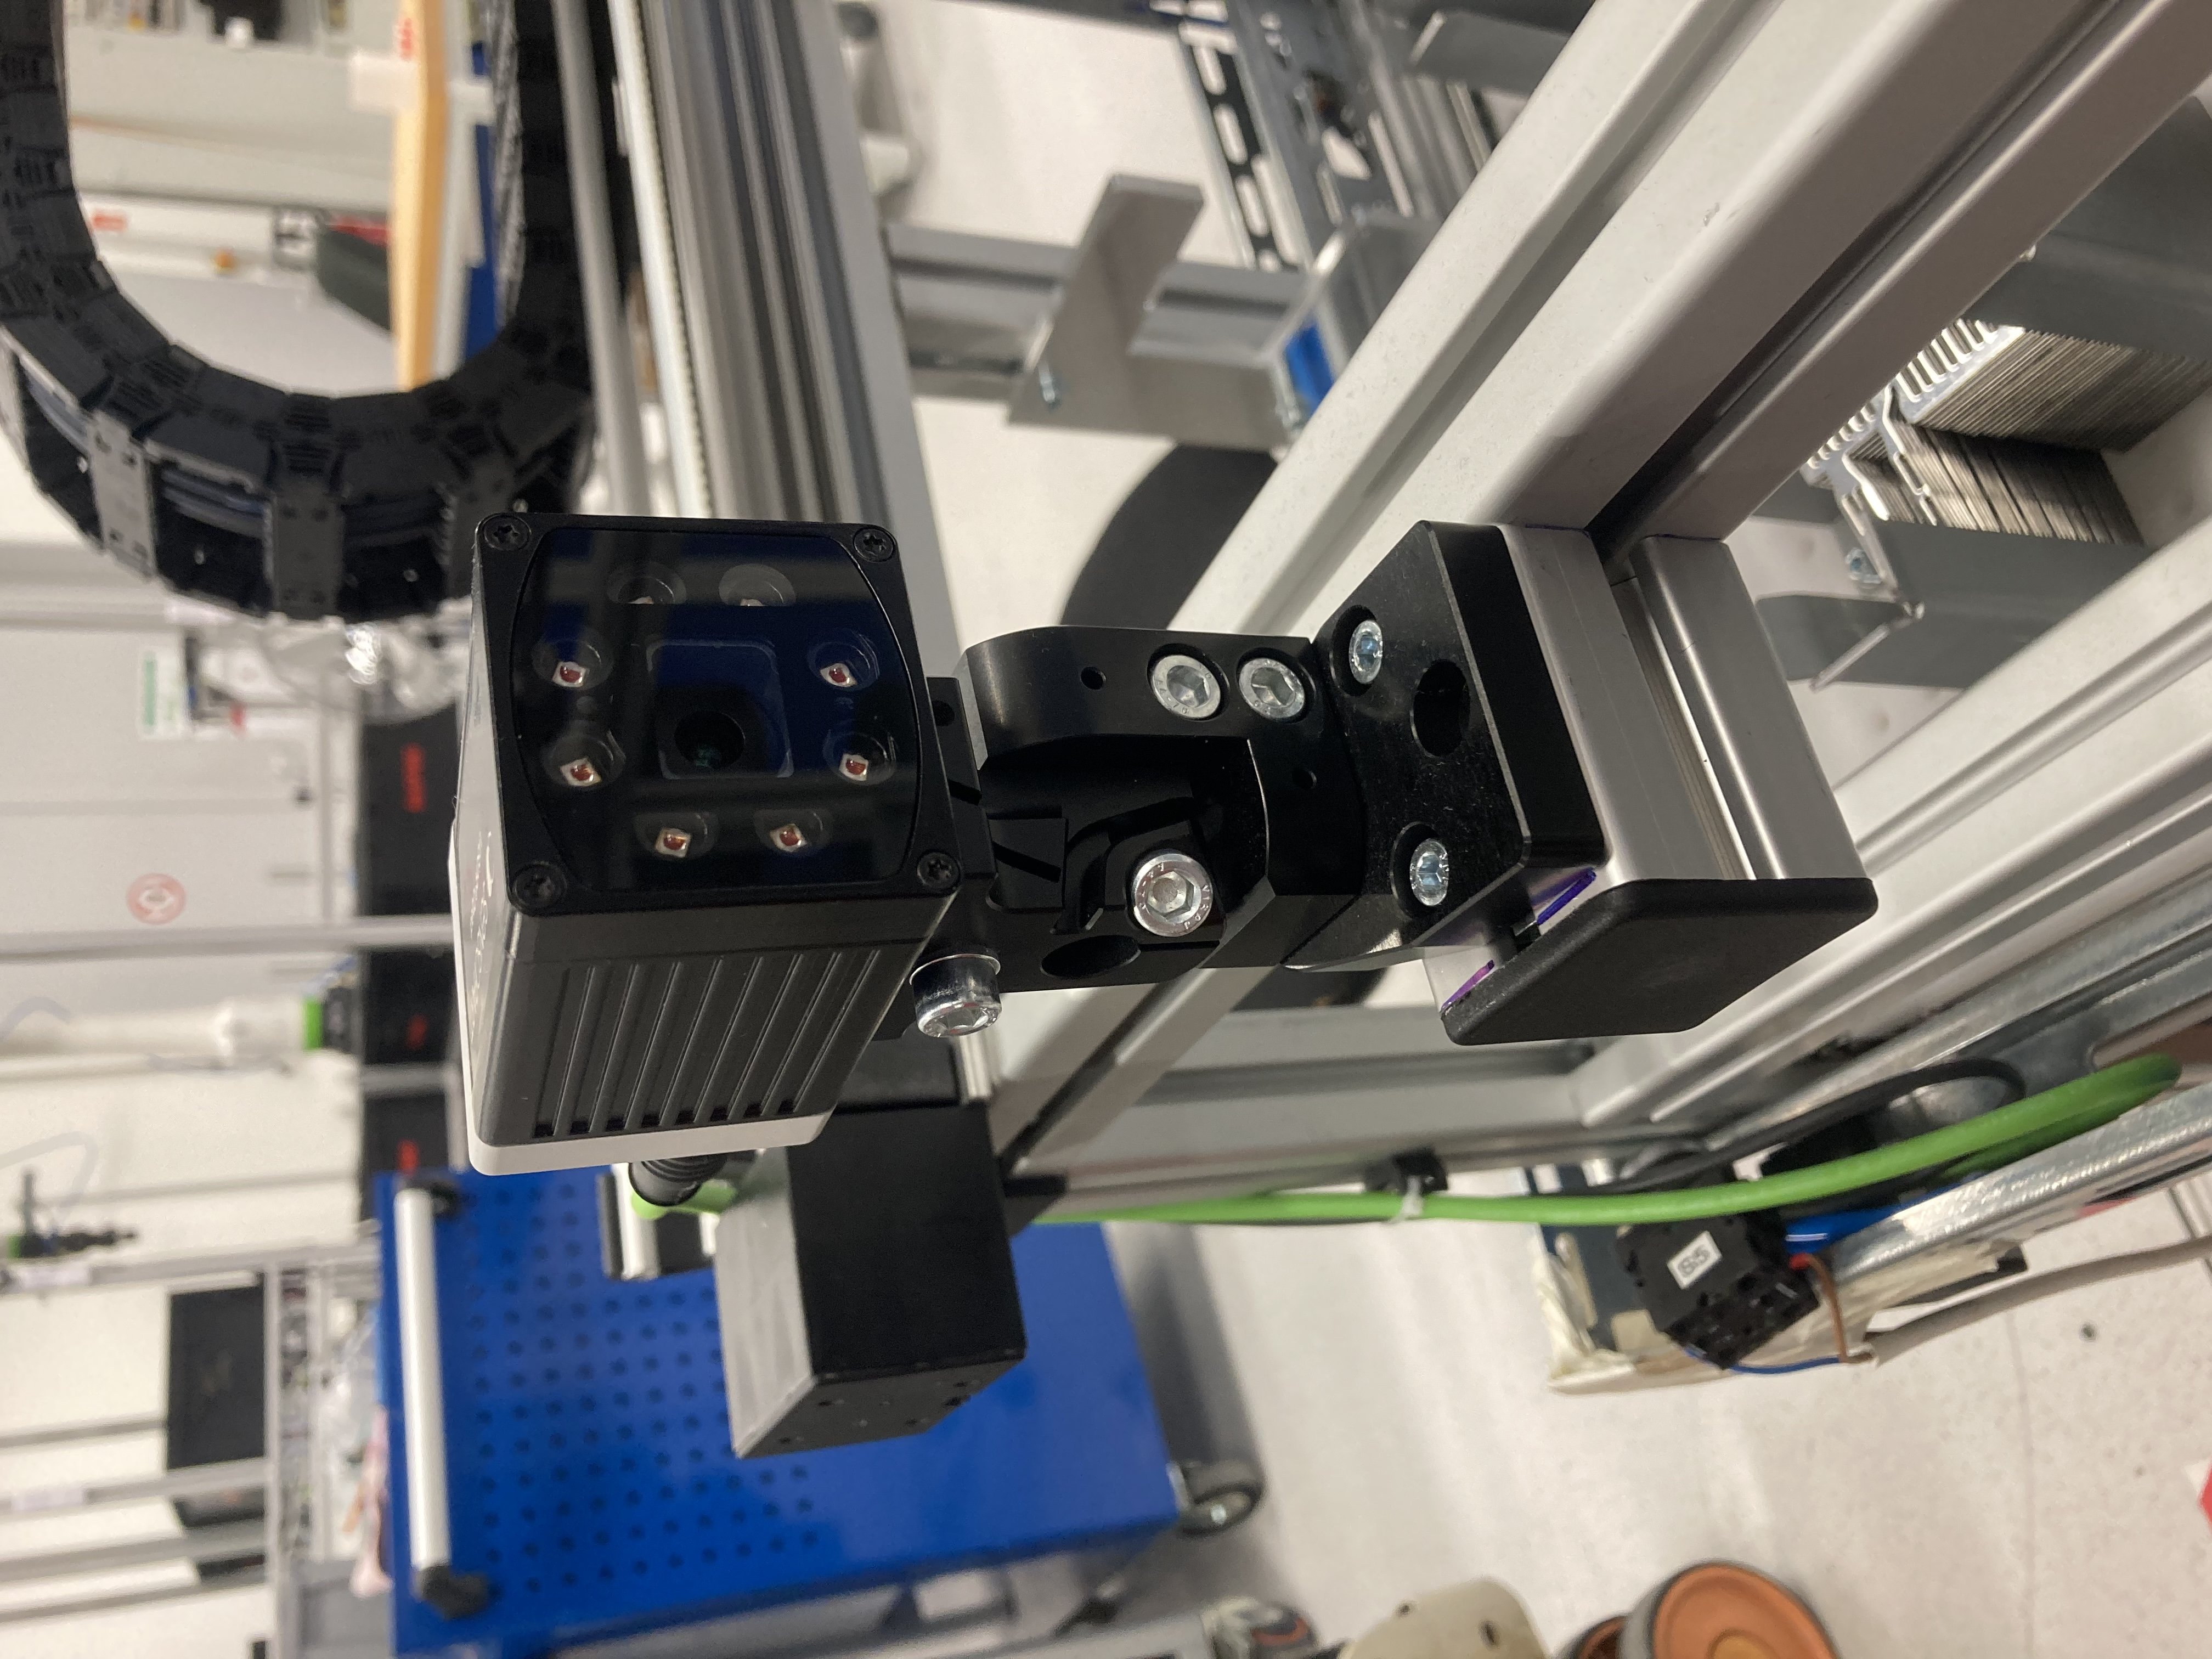
\includegraphics[width=\textwidth, angle=-90]{figures/inspection-camera.jpg} % Replace with your image file
            \caption{}
            \label{fig:inspection-camera}
        \end{subfigure}\hspace{-1.5cm}
        \begin{subfigure}{0.5\textwidth}
            \centering
            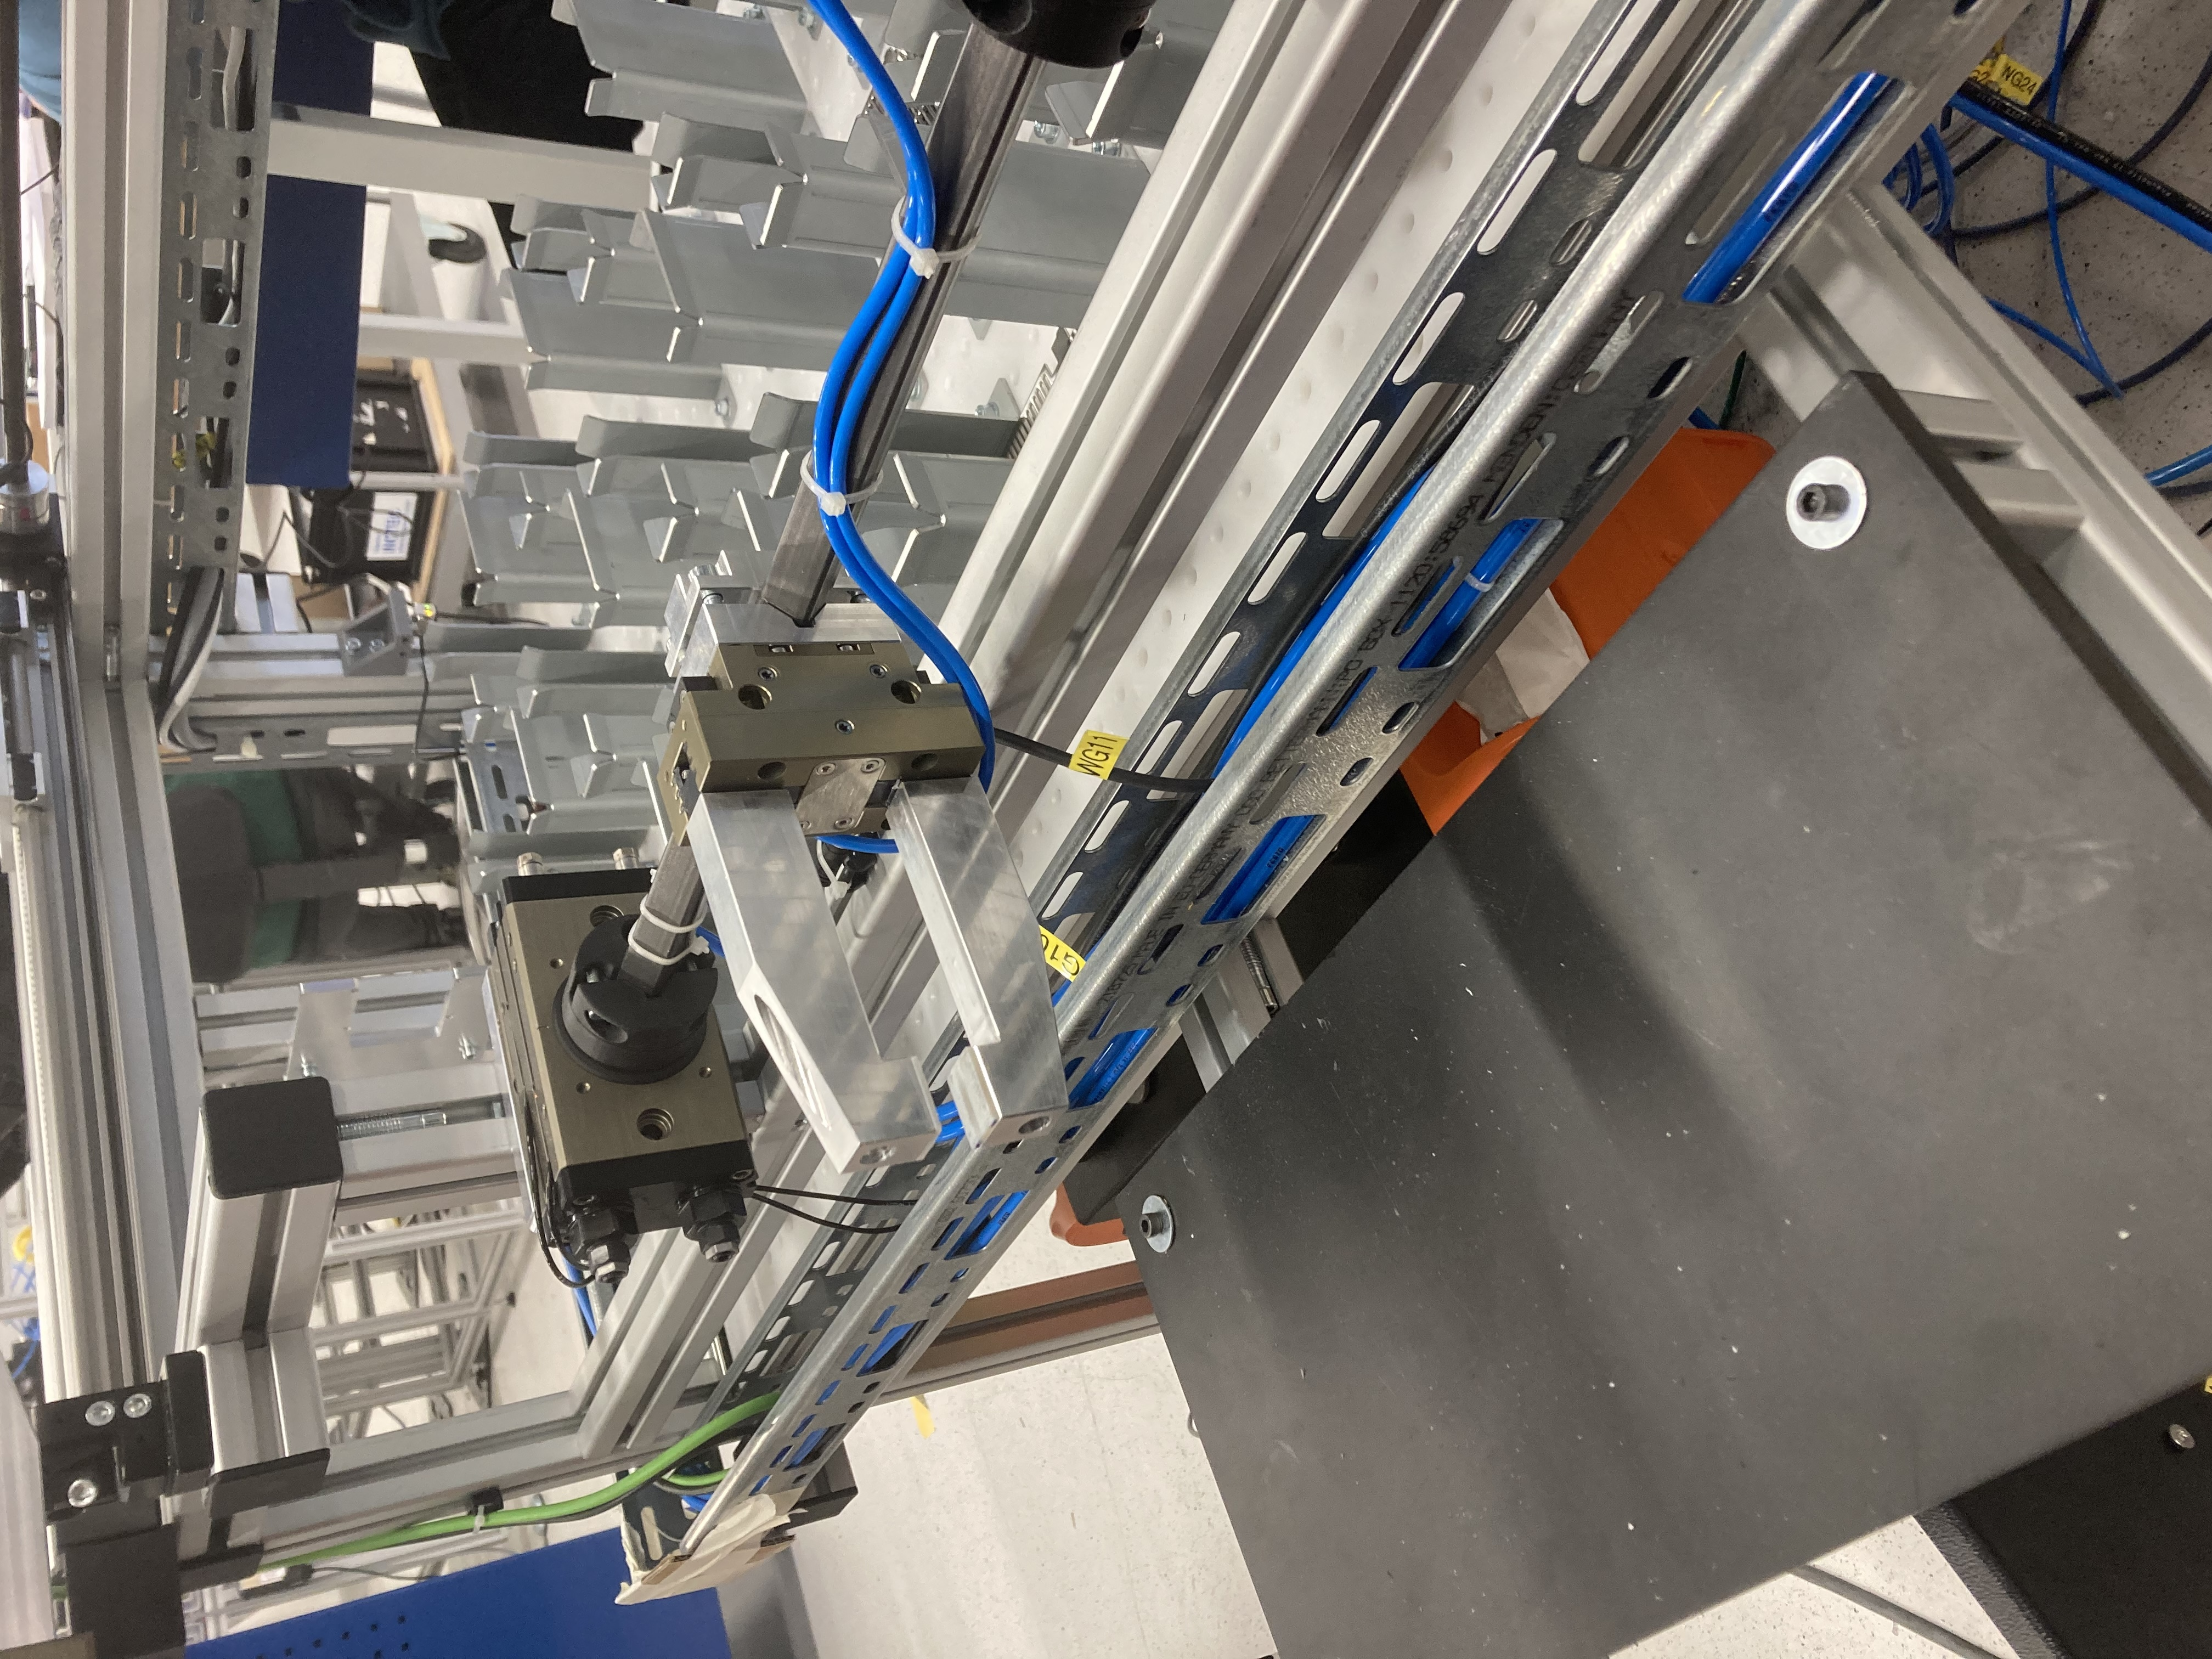
\includegraphics[width=\textwidth, angle=-90]{figures/unloading-station-gripper.jpg} % Replace with your image file
            \caption{}
            \label{fig:unloading-station-gripper}
        \end{subfigure}
        \caption{\parbox[t]{12cm}{Unloading station installations. a) Inspection Camera b) Pneumatic parallel gripper with pneumatic swivel unit}}
        \label{fig:unloading-station-installation}
    \end{figure}
    
    \item As with the robot unit, different grippers (vacuum grippers, magnetic grippers, etc.) can be
    installed very quickly using a manual quick-change system, depending on the type of sheet metal part.
    \item After the gripper has unstacked a raw sheet, it is transferred to a pneumatic 180° swivel unit as shown in figure \ref{fig:unloading-station-gripper}, which in
    turn is equipped with a pneumatic parallel grippers. From
    there, the raw sheet is finally picked up by the robot unit described in the previous subsection \ref{subsec:robot-unit} after the
    exact position has been determined with the camera on the robot. In order to achieve reliable and
    precise positioning, a dark material is installed as background below the swivel unit. 
    \item As there is ample space between robot and unloading station, the inspection camera is installed directly on the unloading station as shown in figure \ref{fig:inspection-camera}.
    The robot comes in front of inspection camera after each bending to get the bending angle.
    \item All electronic
    components such as fuses, power supply units, etc. of the entire mobile robot unit, \textit{i.e.} not just those of
    the unloading station, are installed in several control cabinets below the gantry. This allows the
    unloading station to be used more flexibly later on different sheet metal bending machines. The same is
    planned for the pneumatic components such as switching valves, pressure regulators, pressure
    gauges, etc. Due to the flexibility and the space still available, the KR controller will also be
    placed in the back-side of this station.
    \item The front panel of unloading station has an HMI, an emergency stop button and the robot's teach pendant. Since the robot auto-starts the program
    when the power is turned on, the teach pendant is not used during operation. However, it is placed there for debugging or testing a new robot program.
    \item An HMI control unit from Siemens is installed for the operation (start, pause, stop, etc.) of the entire robotic workcell and as
    a source of information about relevant process values, such as the number of sheets processed or failed in the current batch as shown in figure \ref{fig:simatic-hmi} 
    
    \begin{figure}[h]
        \centering
        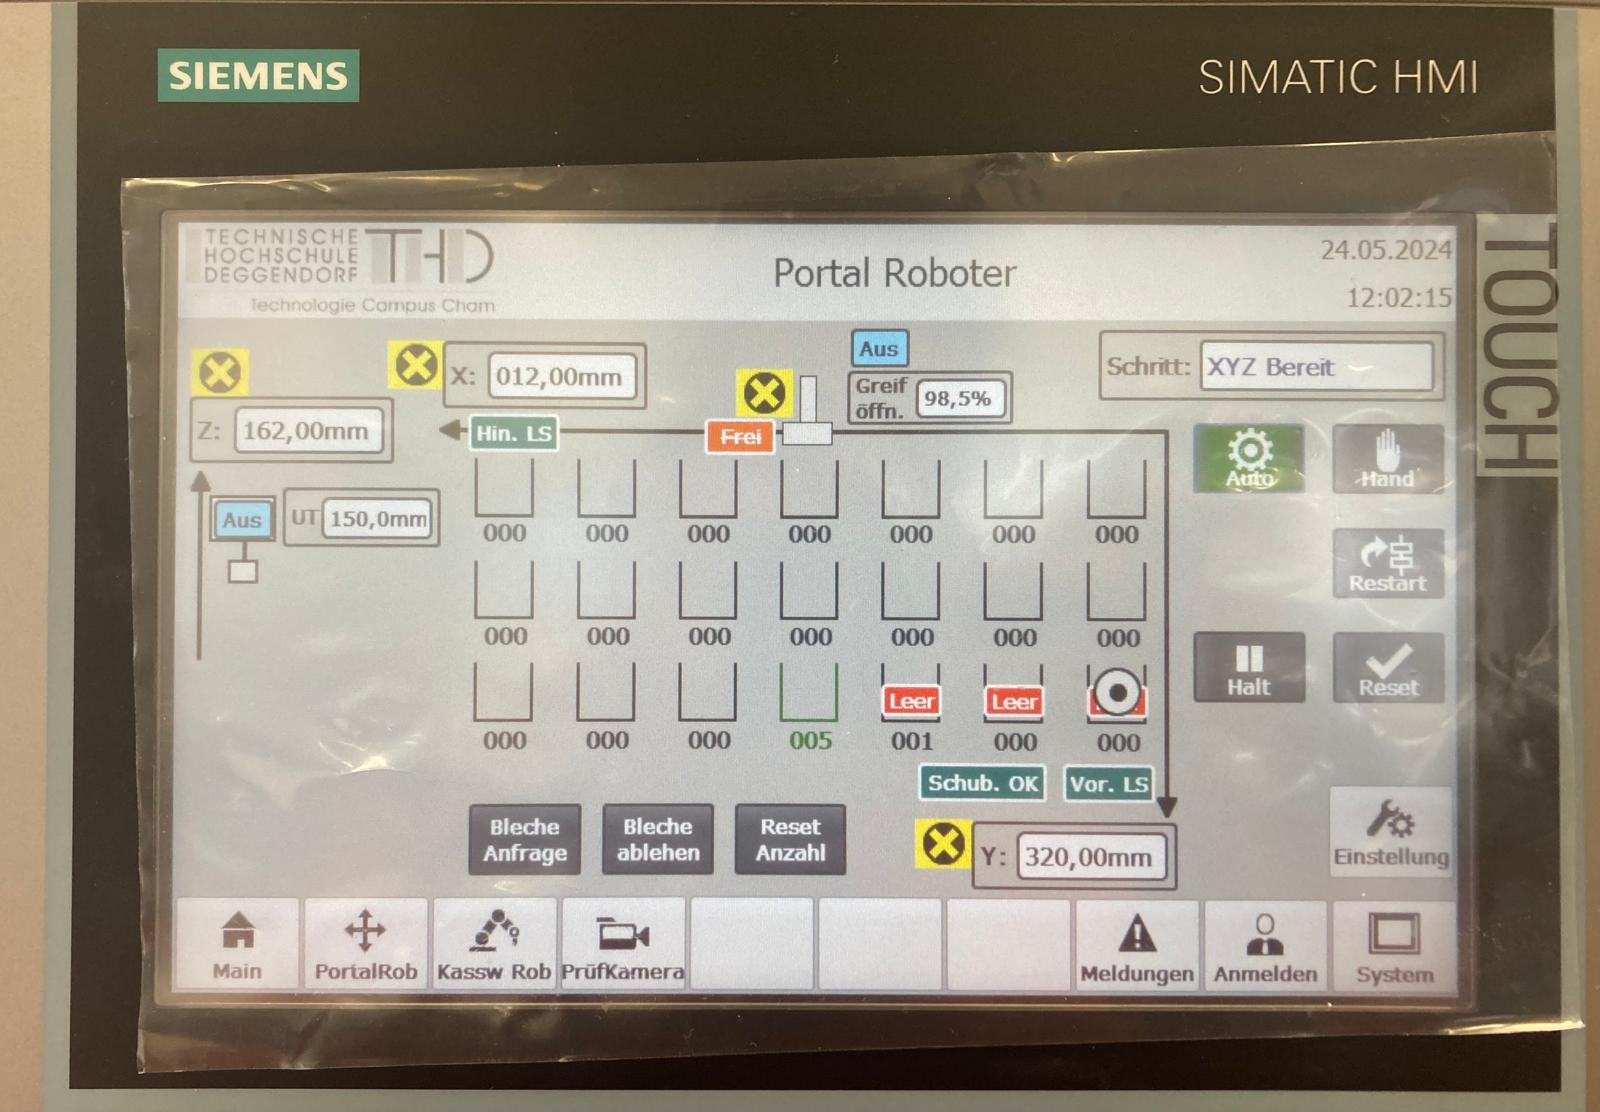
\includegraphics[width=0.5\textwidth]{figures/simatic-hmi.jpeg}
        \caption{HMI showing the sheet available in the unloading station}
        \label{fig:simatic-hmi}
    \end{figure}

    The protective fence is attached with
    the unloading station, but contains a recess so that the HMI can be used at all times.
\end{enumerate}











